%qqqqqqqqqqqqqqqqqqqqqqqqqqqqqqqqqqqqqqqqqqqqqqqqqqqqqqqqqqqqqqqqqqqqqqqqq
%Quote
\begin{savequote}[50mm]
‘‘Equipado con sus cinco sentidos, el hombre explora el universo alrededor 
suyo y llama a esta aventura Ciencia’’ 
\qauthor{Edwin Hubble}
\end{savequote}
%*************************************************************************




%#########################################################################
\chapter{Preliminares}
\label{cha:Introduction}

 
‘‘¿Cuál es nuestro lugar en el cosmos?’’ Esta es una de las más simples
y trascendentales preguntas que han acompañado a los seres humanos
desde su propia existencia, además, potenciada por nuestra curiosidad innata
nos ha conducido a tener una imagen relativamente completa y 
estructurada de nuestro universo. A pesar de lo anterior, esta entendimiento 
es relativamente actual en la historia de la humanidad, tanto que la 
astronomía solo es considerada una disciplina científica rigurosa después 
del siglo diecisiete.


%#########################################################################





%*************************************************************************
%Prehistory
\section{Prehistoria}
\label{sec:Prehistory}


En la mayoría de disciplinas científicas un avance teórico importante 
viene acompañado de una significativa mejora técnica e instrumental, es 
por esta razón que al comienzo del siglo diecisiete Johannes Kepler pudo 
establecer sus tres conocidas leyes de movimiento planetario, basadas en 
los precisos datos de cuerpos astronómicos computados por Tycho Brahe. Este 
evento fue de gran importancia en la historia de la astronomía y la ciencia 
moderna debido a que fue el primero de muchos golpes contra la aceptada
noción antropocéntrica del cosmos. A pesar de estas leyes de Kepler 
constituían la prueba más crucial del modelo heliocéntrico de Nicolás 
Copérnico, fue solo hasta 1685 cuando Isaac Newton formuló su ley de 
gravitación universal (de las cuales pueden ser derivadas todas las leyes
de Kepler) cuando los astrónomos pudieron tener un conjunto de herramientas
teóricas suficientemente potentes para comenzar una discusión seria y 
profunda de la naturaleza real de nuestro universo a escalas mayores que el 
sistema solar, inaugurando así las \textit{ciencias de la gravedad} 
\cite{longair2008}.


Después de la formulación de la gravitación universal, el siguiente avance
teórico importante en esta área viene en los siglos dieciocho y diecinueve
con el desarrollo de la mecánica clásica, como el formalismo lagrangiano y
hamiltoniano, y de poderosas herramientas numéricas. Todos estos logros
impulsaron el estudio de temas claves como el problema de muchos cuerpos,
permitiendo un profundo entendimiento de la dinámica de sistemas 
gravitacionales complejos, tales como sistemas planetarios, cúmulos estelares,
etc.


Paralelo a lo anterior, en el lado observacional comenzaba a surgir la idea
de \textit{universo isla}, del cual evolucionaría el concepto de galaxia. 
Todo esto fue potenciado enormemente por el desarrollo del telescopio, 
permitiendo además entender que la galaxia es tan solo una gran colección
de estrellas tal como nuestro sol. Fue muy notable el trabajo pionero de 
William Herschel, quien intentó realizar un mapa de nuestra galaxia 
determinando distancias a partir de la asunción de estrellas con la misma
luminosidad intrínseca y la ley de inverso cuadrado para el decaimiento de 
la intensidad (figura \ref{fig:HerschelModel}). Aunque sus resultados
fueron muy imprecisos debido a la asunción incorrecta en que se basaban, 
la importancia de este trabajo radica en el reconocimiento de una estructura
(discoidal) de nuestra galaxia.


%.........................................................................
%Herschel Model of Our Galaxy
\begin{figure}[htbp]
	\centering
	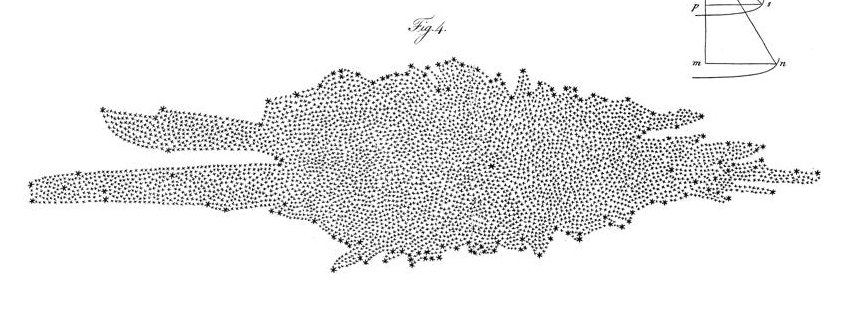
\includegraphics[width=1.0\textwidth]
	{./figures/1_introduction/Herschel_Model.png}
	
	\caption{\small{Modelo de William Herschel para nuestra galaxia, basado
	en un conteo de estrellas y la asunción de igual luminosidad 
	\cite{Herschel1785}.}}
	
	\label{fig:HerschelModel}
\end{figure}
%.........................................................................


Otra importante cuestión observacional que estaba emergiendo en esa época
fue sobre la existencia de otros \textit{universos islas} tal como el nuestro.
Era ya bien conocida la existencia de cuerpos extendidos en el cielo que no
se acomodaban satisfactoriamente a la definición de estrellas o planetas,
tales como nebulosas, discos planetarios y galaxias. Incluso William Herschel
y su hijo John Herschel contribuyeron con la realización de un gran catálogo
(para la época) de cuerpos extendidos conocido como \textit{Catálogo de 
Nebulosas y Cúmulos de Estrellas} y una versión extendida terminada por
John Dreyer en 1888, \textit{Nuevo Catálogo General de Nebulosas y Cúmulos
de Estrellas}, los cuales junto con el \textit{Índice de Catálogos} de 
1895 y 1908 constituyen una amplia colección de cuerpos ampliamente usados
en la astronomía actual, referidos con sus abreviaciones en inglés \textit{NGC}
y \textit{IC} respectivamente \cite{longair2008}. A pesar de todos estos
logros observacionales, la naturaleza real de estos objetos era un completo 
misterio, especialmente si ellos eran objetos dentro de nuestra propia 
galaxia o eran sistemas completamente independientes.


Esta última cuestión permaneció hasta el siglo veinte, y junto con el tamaño
real del universo constituyeron los dos grandes temas tratados en el 
conocido \textit{Gran Debate}, también denominado \textit{Debate de 
Shapley-Curtis}. Un importante evento en la historia de la astronomía donde
los astrónomos Harlow Shapley y Herber Curtis sometieron respectivamente 
diferentes argumentos a favor y en contra de la pertenencia de esos objetos
a nuestra galaxia y si la Vía Láctea era todo nuestro universo 
\cite{Curtis1921} \cite{Shapley1921}. A pesar de todo, sus argumentos fueron 
poco concluyentes y la solución a estos problemas debió esperar hasta 1924 
cuando Edwin Hubble midió la distancia a la galaxia de Andrómeda (M31 o 
NGC 224) y demostró incuestionablemente la verdadera naturaleza extragaláctica 
de este objeto, y en años posteriores para los demás \cite{Hubble1926}. 
Este logro junto con la verificación observacional de la expansión del 
universo (también debida a Hubble) fueron el comienzo de la cosmología 
observacional moderna.


También sucedió en este mismo siglo un evento clave para las modernas 
\textit{ciencias de la gravedad}, Albert Einstein formuló su Teoría
General de la Relatividad \cite{Einstein1916}, cambiando completamente 
la concepción previa de espacio y tiempo y llegando así a nuestro paradigma 
cosmológico actual.


%*************************************************************************




%*************************************************************************
%The current cosmology picture
\section{El Paradigma Cosmológico Actual}
\label{sec:TheCurrentCosmologyPicture}


Las bases teóricas para la relatividad general comenzaron a surgir con el 
auge de las geometrías no Euclidianas en el siglo diecinueve y comienzos 
del veinte, cuando fue demostrado que el quinto postulado de Euclides no 
era necesario para construir geometrías autoconsistentes y llegando así a 
las geometrías no planas (ver figura \ref{fig:NonEuclidean}). En especial 
fueron destacables los trabajos de Nikolai Lobachevsky (padre de las 
geometrías no Euclideas) y Bernhard Riemman, fundador de la geometría 
Riemanniana.


%.........................................................................
%Herschel Model of Our Galaxy
\begin{figure}[htbp]
	\centering
	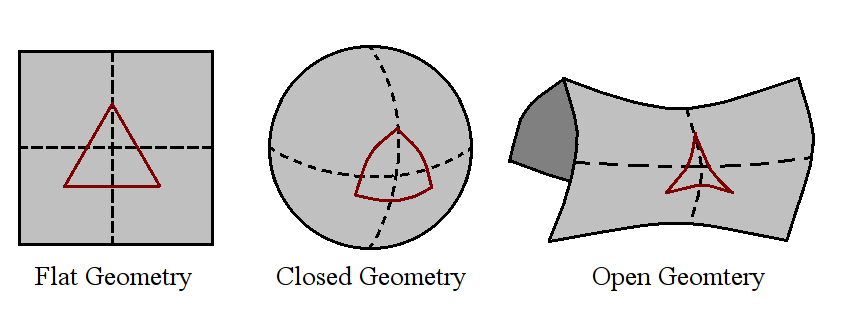
\includegraphics[width=0.9\textwidth]
	{./figures/1_introduction/Non_Euclidean.png}
	
	\caption{\small{Diferentes geometrías con variación del quinto postulado 
	de Euclides.}}
	
	\label{fig:NonEuclidean}
\end{figure}
%.........................................................................


A pesar de que estos primeros desarrollos en geometría habían dado lugar a
fuertes discusiones sobre el tipo de geometría del universo, los conceptos 
de espacio y tiempo eran aún interpretados de forma absoluta y más aún, su 
conexión con la gravedad completamente ignorada. Es por esta razón que 
la formulación de la Relatividad General abrió la puerta a toda nuestra
comprensión moderna.


Una vez obtenidas las ecuaciones de campo métrico de la Relatividad General
fue posible construir modelos globales y autoconsistentes del universo. Un
primer intento se debe al propio Einstein, quién formuló con influencia 
de su propia creencia un modelo de universo estático y cerrado. Para lograr 
esto debió hacer uso de la bien conocida constante cosmológica para 
contrarrestar la expansión/contracción natural de las soluciones que da
la teoría.


Pocos años después Aleksander Friedmann demostró en una serie de dos 
artículos un conjunto de soluciones para universos cerrados o hiperbólicos
que se expanden desde una singularidad \cite{FriedmanA} \cite{FriedmanB}, 
lo que concordaba perfectamente con las observaciones realizadas por Hubble 
para el corrimiento al rojo de galaxias distantes. Debido a esto, la 
inclusión de la constante cosmológica para soluciones estacionarias es 
conocido históricamente y reconocido por él mismo, como el mayor ‘‘resbalón’’ 
de la vida de Einstein. Después de esto hubo un aumento considerable en las 
investigaciones sobre la naturaleza del universo acorde a este tipo de 
soluciones, como la dinámica a gran escala, la geometría global y la 
medición precisa de un conjunto de parámetros cosmológicos de los modelos.


El siguiente avance importante viene con la formulación de la teoría del 
Big Bang por parte de George Gamow, donde se propone que los primeros
estadios del universo habían sido muy densos y calientes, partiendo de una
singularidad y llegando a los estadios tardíos donde el universo se ha 
estado expandiendo y enfriando, acorde a la solución de Friedmann. Una
de las primeras consecuencias de esta teoría es la nucleosíntesis temprana,
donde reacciones de fusión de hidrógeno produjeron elementos más pesados 
a partir del Hidrógeno, tales como Helio y Litio, lo cual no puede ser 
explicado a partir de reacciones de fusión en estrellas. La nucleosíntesis
temprana fue demostrada por Ralph Alpher y Robert Herman y ha sido 
corroborada observacionalmente de forma muy precisa.

\
%.........................................................................
%Cosmic Background Radiation
\begin{figure}[htbp]
	\centering
	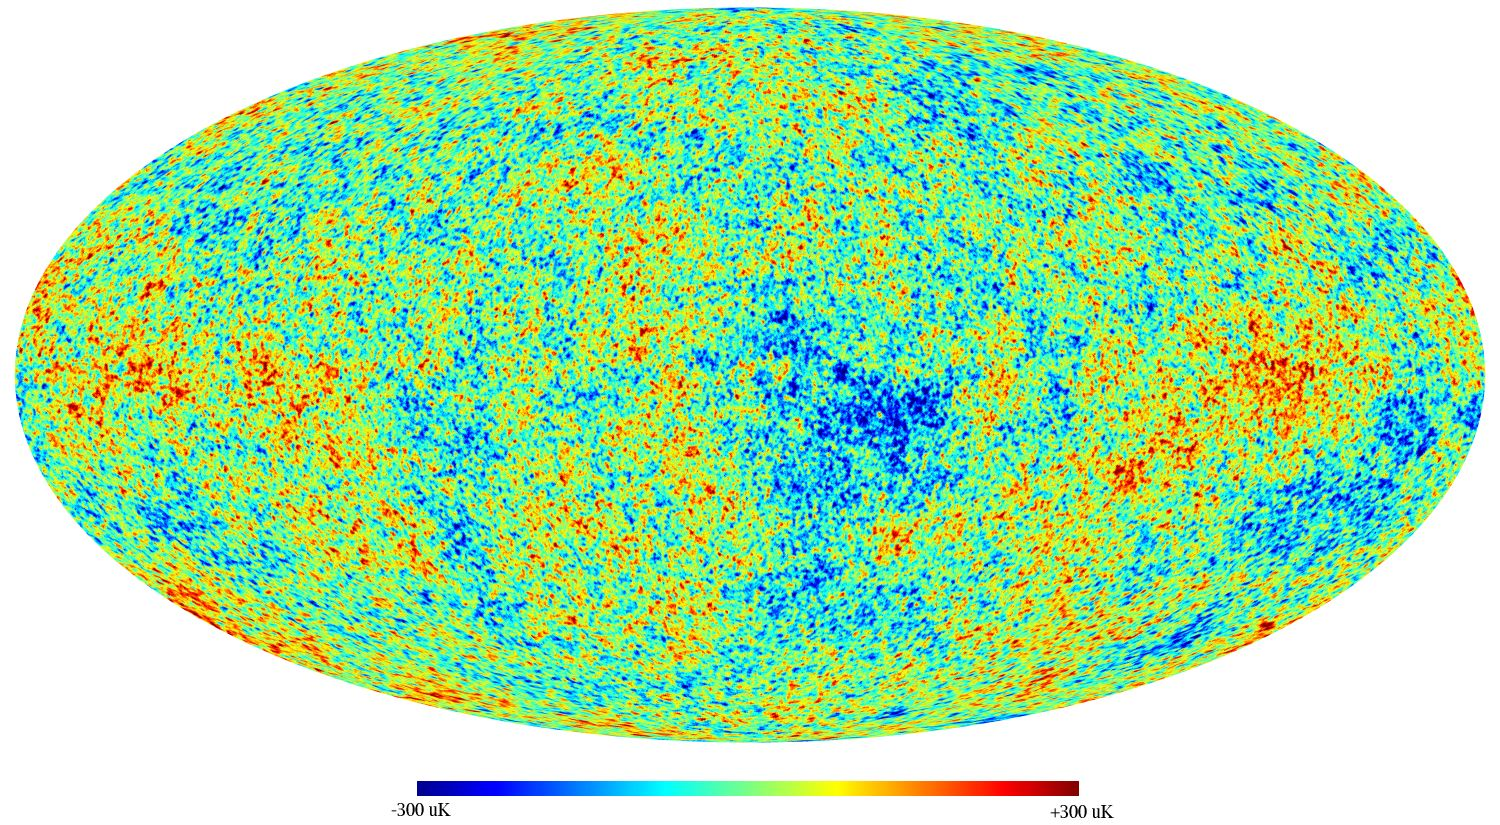
\includegraphics[width=0.8\textwidth]
	{./figures/1_introduction/CMB.png}
	
	\caption{\small{Radiación cómica de fondo. Tomado de 
	\url{http://upload.wikimedia.org/wikipedia/commons/3/3c/Ilc_9yr_moll4096.png}}}
	
	\label{fig:CMB}
\end{figure}
%.........................................................................


La segunda consecuencia del Big Bang es la presencia de un remanente de 
radiación de cuerpo negro del universo temprano, donde debido a la alta 
densidad y temperatura este era dominado completamente por la radiación.
Esto fue corroborado por observacionalmente por Arno Penzias y Robert
Wilson en 1965 con el descubrimiento de la radiación cósmica de microondas
(CBM por su siglas en inglés), donde se midió un espectro de cuerpo negro
de fondo en el universo con una temperatura asociada de $T = 2.725$ K. 
Estas dos predicciones de al teoría del Big Bang han hecho que sea 
adoptado como parte del modelo cosmológico estándar.


Uno de los primeros problemas originados con el descubrimiento de la 
radiación cósmica de fondo es el problema de horizonte. Esto surge debido
la alta isotropía angular medida en el espectro de radiación de fondo (ver 
figura \ref{fig:CMB}), indicando una conexión causal entre regiones tan 
apartadas del universo, que en principio no deberían estarlo. La solución 
al problema fue propuesta por Alan Guth en 1980 y se denomina teoría de 
inflación. En esta se postula una expansión exponencial en el universo 
temprano impulsada por un campo escalar (inflatón). En este periodo de 
expansión se magnificaron las fluctuaciones cuánticas del vacío de todos 
los campos presentes en el universo, produciendo así pequeñas perturbaciones 
en el campo de densidad de las cuales luego evolucionarían las estructuras 
a gran escala de la actualidad. Acorde a esto, la teoría inflacionaria 
también explica satisfactoriamente el problema de pequeñas perturbaciones 
en el universo primigenio, convirtiéndose así en parte del paradigma 
cosmológico actual.


La existencia de la materia oscura fue propuesta desde principios de la 
década de 1930, primero por parte de Jan Oort en 1932 y luego por Fritz
Zwicky en 1933, para dar cuenta de materia no lumínica en galaxias y 
cúmulos galácticos que se manifiesta de forma dinámica. A pesar de esto 
su naturaleza física era completamente desconocida. En 1984 Joel Primack,
George Blumenthal, Sandra Moore y Martin Rees propusieron un modelo de 
materia oscura fría (CDM por sus siglas en inglés), para el cual la 
materia oscura corresponde a un tipo de partícula no relativista que solo
interactua gravitacionalmente y de forma muy débil electromagnéticamente.
Bajo este esquema es posible demostrar que la formación de estructuras a 
gran escala se da de forma jerárquica en un proceso de \textit{top-down},
en el cual las estructuras más pequeñas se forman primero y a partir de 
agrupación de estas se forman las estructuras de gran escala, lo que ha 
sido verificado observacionalmente por surveys de galaxias (ver sección
\ref{sec:CosmologicalObservations}).


En la década de 1990 algunas observaciones cosmológicas comenzaron a 
mostrar una rata de expansión acelerada para el universo, lo que solo 
puede ser explicado (ver subsección \ref{subsec:SimpleSolutionsOfTheUniverse})
con la inclusión de una constante cosmológica en las ecuaciones de campo
de la relatividad general. El término de energía oscura fue acuñado debido 
a que esta constante puede tomarse como una densidad física de energía que
actúa con una presión negativa, impulsando así la rata de expansión del 
universo, a pesar de esto su naturaleza física es completamente incierta.
Mediciones precisas muestran que actualmente el universo está dominado por 
este tipo energía, alcanzando el $70 \%$ del total de materia-energía 
presente en el universo. Eso último completa el paradigma cosmológico 
actual y es denominado modelo estándar $\Lambda$CDM o modelo de 
concordancia.

\
%.........................................................................
%Local Group
\begin{figure}[htbp]
	\centering
	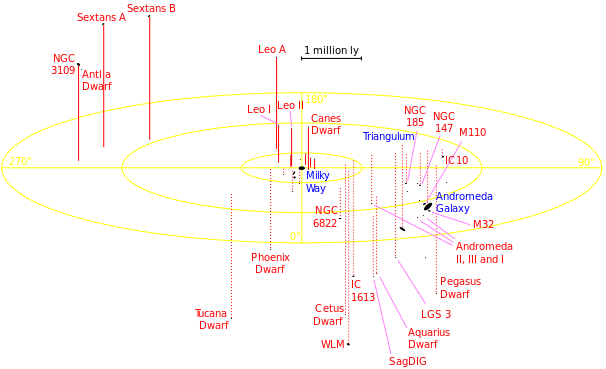
\includegraphics[width=1.0\textwidth]
	{./figures/1_introduction/LocalGroup.png}
	
	\caption{\small{Grupo Local. Tomado de 
	\url{http://commons.wikimedia.org/wiki/File:Local_Group.svg}}}
	
	\label{fig:LocalGroup}
\end{figure}
%.........................................................................


El grupo local es un sistema de aproximadamente 30 galaxias que interactúan
gravitacionalmente entre ellas y evolucionan de forma relativamente aislada
de otras estructuras a gran escala, con la Vía Láctea y Andrómeda como 
miembros más representativos (ver figura \ref{fig:LocalGroup}).


La importancia del grupo local en un contexto cosmológico se debe a que es
la estructura a gran escala más conocida, permitiendo así verificar las 
predicciones del modelo cosmológico estándar. Entre los problemas actuales
en esta línea destacan la sobreabundancia de galaxias satélites para la 
Vía Láctea, la conexión entre los flujos de las nubes de Magallanes y la
galaxia de Andrómeda, fuerzas de marea en el grupo local, la cinemática 
de Andrómeda y la Vía Láctea en un contexto cosmológico \cite{forero2013}
y la influencia del entorno cosmológico en la formación de sistemas como
el grupo local.


%*************************************************************************





%*************************************************************************
%Cosmological observations
\section{Observaciones Cosmológicas}
\label{sec:CosmologicalObservations}
	

El auge generado por la era espacial junto con el gran avance tecnológico
de ins\-trumentos de medida y sensores ha potenciado enormemente las 
investigaciones observacionales en cosmología, permitiendo en conjunto con 
los avances teóricos llegar al paradigma cosmológico actual y contrastar los 
diferentes modelos que han surgido. A continuación se presentan algunos de 
los proyectos observacionales más destacados en cosmología y que son 
ampliamente usados en investigaciones actuales.


	%---------------------------------------------------------------------
	%2DF Galaxy Redshift Survey
	\subsection*{2DF Galaxy Redshift Survey}
	\label{subsec:2DFGRS}
	%---------------------------------------------------------------------
	
	
El 2DF Galaxy Redshift Survey (2DFGRS) o sondeo de corrimiento al rojo en 
un campo de 2 grados\footnote{Página oficial del proyecto 
\url{http://magnum.anu.edu.au/~TDFgg/}.}, es un sondeo del corrimiento al 
rojo de un conjunto de galaxias dentro de una área de $1500$ grados cuadrados 
para zonas cercanas al polo sur y norte galáctico esto para evitar la extinción 
provocada por el disco galáctico. Fue realizado por el telescopio de $3.9$ m 
del observatorio Anglo-Australiano entre 1997 y 2002. Entre los principales 
resultados de este sondeo destaca el establecimiento de la estructura local 
a gran escala en torno al grupo local a partir de medidas fotométricas de 
$382\ 323$ objetos para corrimientos al rojo menores a $z=0.3$, también 
destaca la medida del parámetro de densidad de materia no relativista (
oscura + bariónica) en el modelo cosmológico estándar.

	
	%---------------------------------------------------------------------
	%Sloan Digital Sky Survey
	\subsection*{Sloan Digital Sky Survey}
	\label{subsec:SDSS}
	%---------------------------------------------------------------------


El Sloan Digital Sky Survey (SDSS) o sondeo digital del espacio Sloan, al 
igual que el 2DFGRS es un sondeo en corrimiento al rojo del universo a 
gran escala realizado por el telescopio de $2.5$ m en el observatorio Apache 
Point en Nuevo México desde el año 2000.


%.........................................................................
%SDSS
\begin{figure}[htbp]
	\centering
	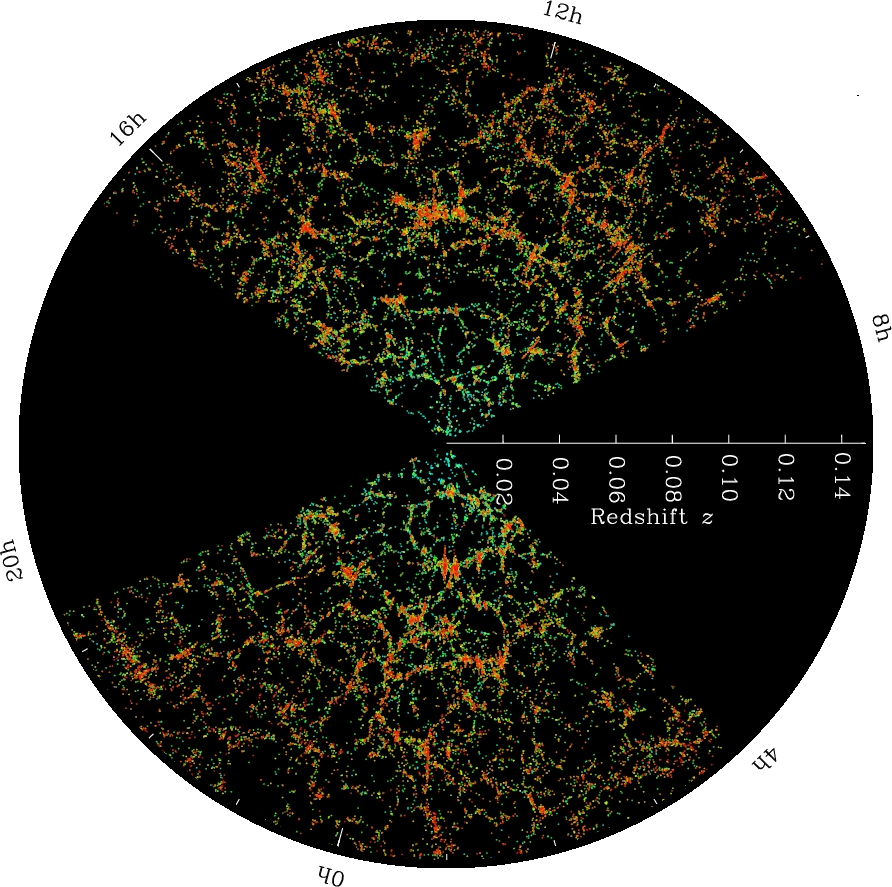
\includegraphics[width=0.6\textwidth]
	{./figures/1_introduction/SDSS.png}
	
	\caption{\small{Mapa del universo a gran escala de acuerdo al Sloan 
	Digital Sky Survey. Tomado de la página oficial del proyecto 
	\url{http://www.sdss.org/}}}
	
	\label{fig:SDSS}
\end{figure}
%.........................................................................


El sondeo cubre una zona significativamente mayor que el 2DFGRS, 
aproxi\-madamente $7500$ grados cuadrados y ha catalogado alrededor de 
$2$ millones de objetos, permitiendo construir un mapa a gran escala del 
universo y percibir por primera vez la estructura de la red cósmica 
(ver figura \ref{fig:SDSS}).
	
	
	%---------------------------------------------------------------------
	%WMAP
	\subsection*{WMAP}
	\label{subsec:WMAP}
	%---------------------------------------------------------------------


La Wilkinson Microwave Anisotropy Probe (WMAP), es una sonsa espacial de 
la NASA lanzada en 2001 y ubicada en el punto de Lagrange L2. Su principal 
objetivo es medir con muy alta precisión los pequeños contrastes de 
temperatura y la polarización de la radiación cósmica de fondo (ver figura 
\ref{fig:CMB}). Aproximadamente cada 2 años la NASA libera los resultados
acumulados obtenidos, referidos como WMAP1, WMAP3, WMAP5, WMAP7 y 
finalmente en el 2012 el WMAP9. Los resultados obtenidos por el WMAP han 
sido hasta el momento la prueba más fehaciente del modelo cosmológico 
estándar $\Lambda$CDM. En especial destacan la medida precisa de la edad del
universo, los diferentes parámetros de densidad, la constante de Hubble, 
la determinación de la geometría global del universo (plana) y la 
confirmación del modelo inflacionario.

\
%.........................................................................
%Cosmological Parameter of WMAP7
\begin{table}[htbp]
\begin{small}
\centering
\begin{tabular}{|c|c|c|c|} \hline
\cellc{\textbf{Parámetro}}		&
\cellc{\textbf{Notación}}		&  
\cellc{\textbf{Valor}}			& 
\cellc{\textbf{Unidades}}					\\ \hline


Edad del Universo  			&	$t_0$			&	$13.75 \pm 0.13$	&	Ga 			\\ \hline

Constante de Hubble			&	$H_0$			&	$71.0 \pm 2.5$		&   km/(Mpc s)	\\ \hline

Parámetro de Hubble			&	$h$				&	$0.71 \pm 0.025$	&   --			\\ \hline

Densidad de Bariones		&	$\Omega_b$		&	$0.0449\pm 0.0027$	&	--			\\ \hline

Densidad de & & & \\
Materia Oscura				&	$\Omega_c$		&	$0.222 \pm 0.026$	&	--			\\ \hline

Densidad de & & & \\
Energía Oscura				&	$\Omega_\Lambda$&	$0.734 \pm 0.029$	&	--			\\ \hline

Densidad de & & & \\
Radiación					&	$\Omega_r$		&$8.24 \times 10^{-5}$	&	--			\\ \hline

Amplitud de & & & \\
Fluctuaciones en $8h^{-1}$ Mpc&	$\sigma^2_8$	&	$0.801 \pm 0.030$	&	--			\\ \hline

Índice Espectral			&	$n_s$			&	$0.963 \pm 0.014$	&	--			\\ \hline
Profundidad Óptica & & & \\
de Reionización 			&	$\tau$			&	$0.088 \pm 0.015$	&	--			\\ \hline
				
Densidad Total & & & \\
del Universo	&	$\Omega_0$		&	$1.080\ \mbox{\scriptsize{$+0.093$}}/ 
										\mbox{\scriptsize{$-0.071$}} $&	--				\\ \hline
\end{tabular}
\caption{Parámetros cosmológicos WMAP7 \cite{WMAP7}.}
\label{tab:CosmologicalParameters}
\end{small}
\end{table}
%.........................................................................


En la tabla \ref{tab:CosmologicalParameters} se tabulan los resultados 
del WMAP7 \cite{WMAP7}, los cuales son ampliamente usados en los siguientes 
capítulos y en especial las diferentes simulaciones cosmológicas presentadas en
los capítulos \ref{cha:N-BodySimulations} y \ref{cha:Results} están basadas
en estos.


%*************************************************************************